\chapter{Understanding}

\keywords{facts and experience, doubt, accumulating facts}

Though we break knowledge into parts and we speak about practice in
gradual steps, understanding happens all at once. Perception is
immediate -- the `Aha!' moment, when the fog clears. While some
information is necessary to begin, we remember that the truth of the
teaching is `to be experienced for oneself'. In meditation practice, the
facts which are useful for us are \emph{here-and-now} facts which we can
know in our present experience.

If we depend solely on external information or simply wait for some
experience to arise, we never arrive at the place where we can stop.
This dependence is exhausting. It keeps creating more doubt and mental
restlessness. Even though we accumulate more facts, we can become
bitter, and this inner feeling of lack grows. It is not more information
that we need. Instead, it is the letting go of that need. Then, we are
able to stop in peace.

\keywords{sense experience, identification}

Memories, perceptions and expectations create a tangible force which
pushes and pulls on us. While the experiences themselves disappear, the
compulsion never rests: we merely want the next one. How can these
phenomena be so convincing that they keep pulling us forward? It is
because \emph{we see ourselves in them.} We see them as what we are,
what we were, what we are going to be. And since they keep changing and
breaking up, we continue on and on, expecting the next one.

\clearpage
\null\vfill

\begin{figure}[h]
\caption{Sense Experience and Identification}\label{fig-senses-identification}
\bigskip
\hspace*{-10mm}%
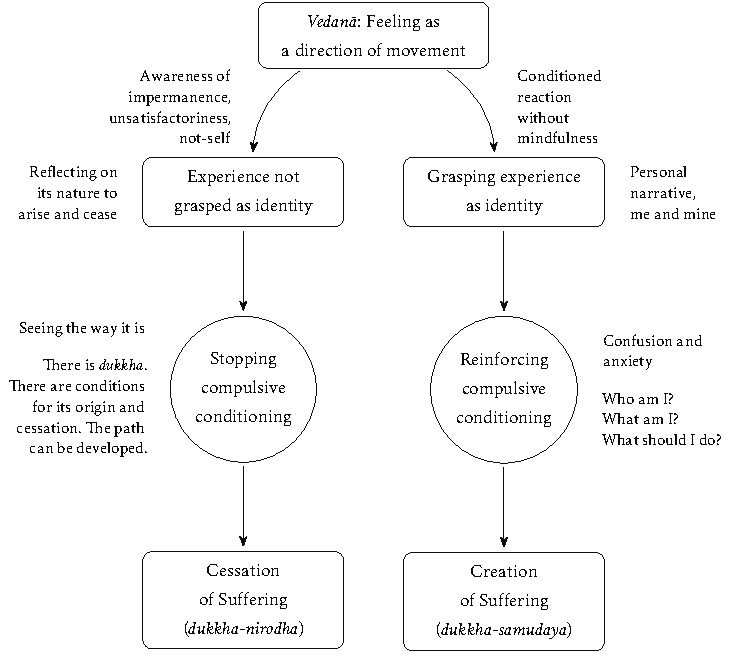
\includegraphics[scale=0.7]{senses-identification.pdf}
\end{figure}

\vfill\null
\clearpage

What if we woke up one morning without any memory of our past? Even in
that state, we would still grasp our experience as \emph{me and mine}.
It might be so disturbing that we would just lie there paralysed with
fear until we were able to grasp some story that could explain where and
who we were. In reality, we don't have to lose our memory to witness
this: missing an important flight connection or any other time when we
can't control our situation can be frightening enough to cause us to
feel this way.

It is humbling to notice how much we take personally, even though
intellectually we know we shouldn't. The Buddha teaches that the mind
continues to construct `me and mine' out of sense-experience until the
impermanence of this experience is fully comprehended. We are taking it
personally if we are convinced that either (1) `This is me', (2) `I am
in this', (3) `I am outside of this', (4) `This is mine', or (5) `I
delight in this'.\footnote{\href{https://suttacentral.net/mn1/en/bodhi}{MN
  1}, The Root of All Things}

Oh, poor mind, why can't you be wiser? To start with, there is little
extra attentional space left when we habitually occupy our minds with
thinking about how to get what we want and complaining about what we
didn't get.

When the sense-base meets a sense-object, if attention is present, we
feel the experience as one of three feelings (\emph{vedanā}), comparable
to a direction of movement: toward the pleasant, away from the
unpleasant, at peace with the neutral. The untrained mind mechanically
follows these established patterns and gets caught up in the underlying
tendencies of passion, hatred and unawareness.

One is said to understand feelings when one understands sense-contact.
As a result one sees the pleasant as painful (due to its ultimately
unsatisfactory nature), sees the painful as a dart (to be removed or
endured skilfully), and sees the neutral as impermanent (not being
lulled to unawareness).

This implies we don't conceive them as `me and mine'. We know them, but
the knowledge is not \emph{ours}. They don't belong to a person who
\emph{has} the feeling.

\begin{quote}
Having fully understood feelings,\\
He is taintless in this very life.\\
Standing in Dhamma, with the body's breakup\\
The knowledge-master cannot be reckoned.

\bigskip

\quoteRef{%

\href{https://suttacentral.net/sn36.5/en/bodhi}{SN 36.5}, Should Be Seen

}
\end{quote}

\keywords{thinking, being burdened, sense-restraint}

We can think a lot about this, but if we are trying to understand it
analytically, we will only give ourselves a headache. This understanding
has to be developed through the body: a good place to start is through
practising sense-restraint.

We guard the sense-doors. Clear comprehension will keep a space, a gap
between our awareness and its contents. When seeing a form, hearing a
sound, etc. we don't grasp at the experience as a whole, or at a
particular feature we like or dislike. We might like the experience, but
we don't become enchanted by it. We might dislike it, but we don't work
up anger over it. It helps to maintain an anchor, a stable point, which
informs our wisdom faculty, such as the sensation of breathing or a
broad awareness of the body. If not the breath, it also works well to
notice an aspect of your current activity, such the touch of the pen as
you write, the pressure of feet on the ground or other sensations of the
body.

This body-based practice is more simple than an intellectual approach.
It collects our mental energies and, with natural rhythm, results in
either calm stillness or thoughtful reflection.

We can notice that we are able to stop and that what we have with us now
is enough. Consider: in terms of objects and information, what have you
actually used today? Although you may own much, for one day, a little is
enough. We don't need as much as we think and relinquishing is not so
much a loss, as a relief from a burden. In this restraint we find
strength and energy which had previously been consumed by distracted
desire. Restraint is always at hand. It is not threatened by external
factors.

This is like learning how to pack less in your backpack for a hike.
After some experience, you can't even comprehend why you needed to carry
so much. Virtue is action that leads to happiness, and it can be
directed towards ourselves. Relinquishment is one such personal virtue.
Understanding informs this virtue, and the happiness born from it
further supports trust in that understanding.

\keywords{ānāpānasati, sense contact, sensation, feeling}

We watch the breathing, and observe how the senses operate. The eye sees
forms, and a sensation appears. The ears hear sounds; the body feels
solidity, hot and cold. With contact, a feeling appears. If there is
contact between a sense-door and a sense-object, sensation is going to
arise. The process doesn't depend on us. When the contact between a
sense-door and a sense-object is broken, sensation ceases. The arising
and ceasing of phenomena dependent on contact -- this was our
experience. Although we may have a measure of control over our
movements, other than that, we don't have a say in the process of
experience: it is not about us.

When we don't notice this, we think that the sensation is ours. If the
sensation feels good, we believe we are going to get something from it
and so we cling to it. This incorrect understanding of things underlies
our neediness and anxiety. When our expectations are confounded, our
tendency is to assume that we did something wrong or that somebody else
made a mistake. We then go and search for some other experience which
will be more right, hoping that this new one doesn't play out like
before.

Observing sense-contact this way, feelings are no longer attractive or
repulsive. Instead, we see that neither inclination is stable or
reliable. This is not numbness. In meditation we turn toward experience,
not away from it. We cultivate attention with sensitive equanimity.
Though we remain alert and responsive to the experience, it no longer
controls and disturbs us. We remain calm.

\clearpage

\begin{figure}[h]
\caption{Sense Contact and Feeling}\label{fig-sense-contact-feeling}
\bigskip\centering
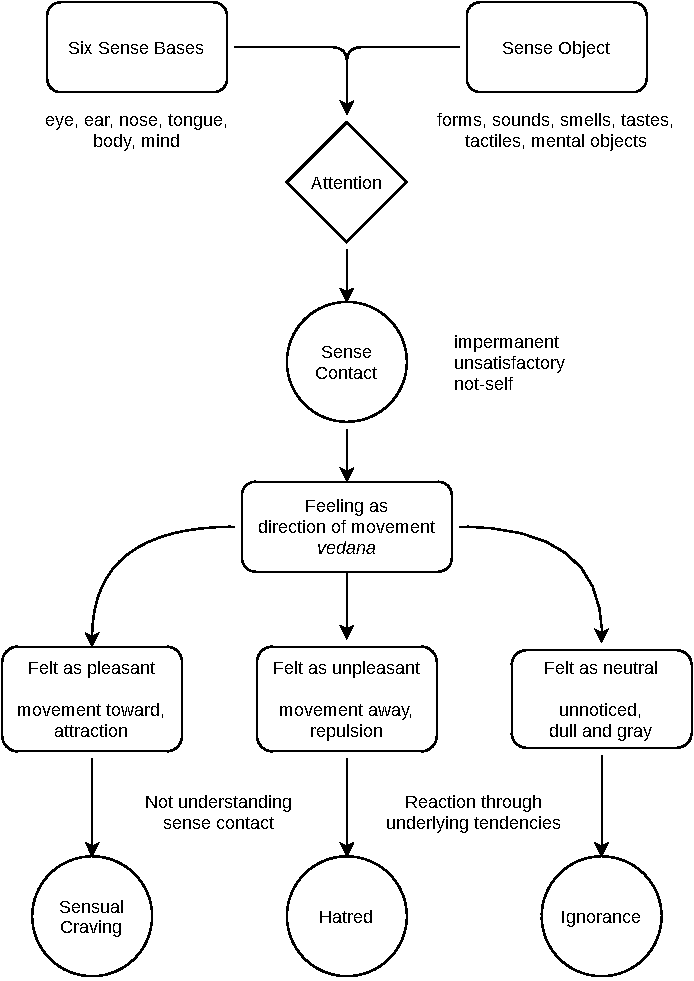
\includegraphics[scale=0.7]{sense-contact-feeling.pdf}
\end{figure}

\clearpage

\keywords{self-narrative}

How does this affect the stories we tell ourselves? A narration is going
on and we are at the microphone. We explain to ourselves that some
feeling was good or bad and we describe how we should think about it.
The central element of this narration is \emph{our feelings}, and its
primary thrust is \emph{to get more of the good ones}.

What happens when we realize that both the good and bad feelings we
experience are unstable and unreliable, and that their arising and
ceasing are not in within our control? Our internal values are
re-ordered, guided by impermanence, rather than craving.

\keywords{changing nature, wise reflection}

Usually we only start to pay attention once we have noticed that
something is wrong, or that something hurts, or that we are suffering.
We don't feel a great need to explain pleasant experiences, do we? We
can use the sense of frustration, the unsatisfactoriness and the
proliferative thinking as a sign to start mindfully investigating.

Mentally take a step back and observe that the experience is a process
which arises, persists in change, and ceases. Ask yourself: `Where in
the body do I feel this sensation? Can I remember when it started? Can I
see how it changes? Can I catch it as the feeling ceases?'

Although we can't control the world around us, our attitude influences
what we see as being free choices. Our perspective opens or closes the
doors toward the actions we see as possible. These actions create the
situations in which we live and influence how we see ourselves therein.
Without reflecting on the nature of our experience, we will be inclined
to see pleasant feelings as a reward and unpleasant feelings as
punishment, and the meaning of our lives will revolve around these. Our
inner world will constantly revolve around the questions of: `Who am I
\ldots{} How do I \ldots{} Why do I \ldots{} What should I \ldots{}' And
doesn't that feel like a burden better left behind?

Wise- and unwise reflection are terms in the \emph{suttas},\footnote{\href{https://suttacentral.net/mn2/en/bodhi}{MN
  2}, All the Taints} making a distinction between a superficial
attention that increases our confusion, and thorough investigation that
leads to clarity and correct understanding. Unwise reflection misses the
signs of impermanence, unsatisfactoriness and not self, hence getting
caught up in taking everything personally. Wise reflection notices these
characteristics of sense-experience, and investigates in line with the
Four Noble Truths.

\keywords{attachment to self, dog tied to a post, reflection}

Have you seen a dog tied up on a leash, running round-and-round its
post? It sits, stands, walks or runs around it, but everything it does
is around that post.\footnote{\href{https://suttacentral.net/sn22.100}{SN
  22.100}, A Leash} This ego-driven proliferation is the same. Although
it keeps us busy, we remain attached to the self at the centre, not
being able to go anywhere else. The leash is the identification and
clinging (\emph{upādāna}), the process of formulating `me and mine' in-,
or around sense-experience, which in truth has no such essential
attribute. This leads us to \emph{unwise} reflection centred on who we
are, what becomes of us, increasing our doubt and confusion.

Questions rooted in `me and mine' are a trap. They drag us on and on
without ever leading to freedom or stopping. If we find ourselves tied
to a post, what are we to do? Cutting the leash suggests itself.

In the context of meditation, reflection doesn't necessarily include all
kinds of thinking. Not all thoughts are productive for insight. In
reflective meditation, we break down our experience into
cause-and-effect processes using the Four Noble Truths\footnote{\href{https://suttacentral.net/sn56.11}{SN
  56.11}, Setting in Motion the Wheel of the Dhamma} as a guide.

This begins with an experience that is personally easy to identify:
suffering, stress, unsatisfactoriness, or \emph{dukkha} in the Pali
language. The direction of thought is not towards \emph{my suffering} as
a personal history, but instead, towards impersonal, natural processes.

\keywords{dukkha}

The starting position is to recognize that stress or suffering \emph{is}
here. As information, this is trivial: yes, there is stress and
suffering in the world. But when we ourselves experience it, we rather
like to pay attention to something else, or we tend to blame somebody
else for it. We will do any number of things rather than becoming
conscious of it and deal with it.

The instruction here is that the way forward is to turn toward suffering
and to investigate it. We seek a way of understanding. This is the First
Noble Truth in the teaching of the Buddha: there is suffering, and the
noble attitude is to turn toward it and understand it.

What do we understand? That this suffering is the result of earlier
causes and didn't arise from nothing. Examining our situation this way,
we are not helpless. Though we may not understand every little aspect of
our condition, it is already a relief to realize that we are, perhaps,
able to change something.

\keywords{origin of dukkha}

The Second Noble Truth points out that the cause of suffering is in
ourselves. It is the wish that experience were otherwise than its nature
dictates. It is our tight clinging to what is impermanent, fragile and
not possible to keep. The suffering, the \emph{dukkha} that we
experience depends on that clinging and thirsty craving. The
instruction, the noble attitude here is to let go of this thirsty
craving and clinging because clinging to transitory experiences is
suffering.

\keywords{cessation of dukkha}

With the cessation of the cause, the result -- the suffering -- ceases
as well. The good news is that the end of suffering is also found within
ourselves.

From this perspective, we can see that the mind creates the kind of
world we live in. If we watch it, we at least have a chance to not make
the situation worse. And who knows, we might make it better?

The Third Noble Truth directs our attention toward this: there is a
solution; we are not obliged to live in bitterness and meaningless
struggle. The advice, the noble attitude is to practise and experience
this for ourselves through understanding and letting go of attachment.
In this way, we allow the suffering to cease.

Even if we can't fully let go right away, it is already a relief to see
that this connection is true: `If I could let go, I wouldn't suffer from
it'. This is already half the work. Until this point, we have been
wandering without a map. But now there is a way forward.

\keywords{path of practice}

The Fourth Noble Truth describes the practice of the path. The Buddha
divided it into eight factors, which incorporate the situations of
everyday life and the development of meditation.

The parts of the Eightfold Path are (1) understanding, (2) intention,
(3) speech, (4) action, (5) livelihood, (6) mindfulness and (8)
concentration. When they are aligned with the truth, we call them
\emph{right}: Right Understanding, Right Intention and so on. Breaking
the path down into parts helps investigation and makes it is easier to
understand, but the path factors strengthen and support one another. The
practice is realized as an integrated whole.

When we most need the practice, we need it \emph{fast.} We can't stop to
count factors. The most useful tools are those which are portable and
most easily accessible in a given situation. When we read and ponder the
meaning, we have time to turn the words this way and that. This is the
stage of study. But mindful attention as an abstract idea doesn't help
much, it is most valuable when practised, when it is at hand in the
present moment.

We always return here. We remember the past and plan for the future, but
remembering is a present experience, and planning is a present
experience. We don't practice meditation for a future state. If we see
understanding, freedom, happiness and overcoming obstacles as some
future state, we only have more burdens. Letting go takes place in the
present, where states are changing without us.
